\documentclass[resume.tex]{subfiles}


\begin{document}
\section{Codage de canal}
$$(n,k,d)_q$$
Lorsque la base est $q=2$ on ne l'affiche pas
\begin{center}
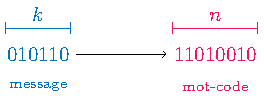
\includegraphics[scale=1,page=1]{drwg_1.pdf}
\end{center}
\begin{center}
\begin{tabular}{c|l}
$k$ & Nombre de bits à transmettre (information)\\
$n$ & Nombre de bits transmis $n\geq k$\\
$d$ & Distance de Hamming
\end{tabular}
\end{center}
\paragraph{Message / information}
$$x=\begin{pmatrix}
x_0 & x_1 & \cdots & x_{n-1}
\end{pmatrix}\in \mathbb{R}^{1\times k}$$
$$x(X)=g_{k-1}X^{k-1}+g_{k-2}X^{k-2}+\cdots+g_1X+g_0$$
\paragraph{Mot-code reçu}
$$y=\begin{pmatrix}
y_0 & y_1 & \cdots & y_{n-1}
\end{pmatrix}\in \mathbb{R}^{1\times k}$$
$$y(X)=g_{n-1}X^{n-1}+g_{n-2}X^{n-2}+\cdots+g_1X+g_0$$
\paragraph{Distance minimale} : $d_{min}$ somme des différences entre deux codes. Pour déterminer la distance minimale on cherche
\begin{itemize}
\item "à l'oeil" entre la liste des mots-codes
\item Le mot-code qui a le moins de $1$ par rapport au mot-code nul (on compte les $1$).
\end{itemize}
Capacité de détection d'erreurs : $d_{min}-1$\\
Capacité de correction d'erreurs : $\left\lfloor\frac{d_{min}-1}{2}\right\rfloor$
\subsection{Liste des codes}
Faire une table avec chaque mot-code et message possible
\begin{center}
\begin{tabular}{cccc|ccccccc}
$X^3$ & $X^2$ & $X$ & $1$ & $X^6$ & $X^5$ & $X^4$ & $X^3$ & $X^2$ & $X$ & $1$\\\hline
0 & 0 & 0 & 0 & 0 & 0 & 0 & 0 & 0 & 0 & 0\\
0 & 0 & 0 & 1 & 0 & 0 & 0 & 1 & 1 & 0 & 1\\
& $\vdots$ & & & & & & $\vdots$
\end{tabular}
\end{center}
Penser à réutiliser des codes ($10$ sera similaire à $1$ mais décalé).

\subsection{Matrice de génération}
Pour déterminer tous les mots-codes, évaluer toutes les entrées possibles.
\subsubsection{Matrice non-systématique}
Pour passer à la matrice systématique on a le droit de
\begin{itemize}
\item Faire des combinaisons linéaires des lignes
\item Permuter des lignes
\end{itemize}
On ne peut pas faire de permutations sur les colonnes.
\subsubsection{Matrice systématique}
La matrice identité se retrouve à gauche
$$G_S=\begin{pmatrix}
\textcolor{RoyalBlue}{I_k} & \textcolor{OrangeRed}{P}
\end{pmatrix}=
\left(\begin{array}{cccc|cccc}
\textcolor{RoyalBlue}{1} & \textcolor{RoyalBlue}{0} & \cdots & \textcolor{RoyalBlue}{0} & \textcolor{OrangeRed}{x} & \cdots & \textcolor{OrangeRed}{x}\\
\textcolor{RoyalBlue}{0} & \textcolor{RoyalBlue}{1} & \cdots & \textcolor{RoyalBlue}{0} & \textcolor{OrangeRed}{x} & \cdots & \textcolor{OrangeRed}{x}\\
\vdots & \vdots & \ddots & \vdots & \vdots & \ddots & \vdots\\
\textcolor{RoyalBlue}{0} & \textcolor{RoyalBlue}{0} & \cdots & \textcolor{RoyalBlue}{1} & \textcolor{OrangeRed}{x} & \cdots & \textcolor{OrangeRed}{x}
\end{array}\right)\in\mathbb{R}^{k\times n}$$
Les $\textcolor{OrangeRed}{x}$ sont des 0 ou 1 en fonction de $P$ (à déterminer pour chaque problème).\\
La forme systématique place les bits au début du mot-code, ce qui permet de décoder très facilement.\\
Pour construire la matrice systématique on peut simplement placer des mots-codes donnés sur les lignes de $G_S$ afin d'avoir la matrice identité au début de $G_S$ (fonctionne car 100 va donner la première ligne de $G_S$, donc la ligne doit être un mot-code).
\subsection{Matrice de vérification}
$$H_s=\begin{pmatrix}
\textcolor{OrangeRed}{P^{T}} & \textcolor{RoyalBlue}{I_{n-k}}
\end{pmatrix}\in\mathbb{R}^{n-k\times n}$$
\subsubsection{Syndrome}
$$S=yH_S^T$$
Si le syndrome est différent de 0, sa valeur donne la position de l'erreur (si le nombre d'erreurs à corriger ne dépasse pas la limite de correction).
$$S=yH_S^T=\big(\underset{\tiny MSB}{s_0}\ s_1\ s_2\ \underset{LSB}{s_3}\big)$$
\subsubsection{Matrice de Hamming ("nombres croissants")}
La matrice de vérification de Hamming permet de déterminer directement la position d'une erreur. Cette matrice est construite avec des nombres binaires croissants (à partir de 1). \textcolor{OrangeRed}{ne pas lire le syndrome directement}
\begin{center}
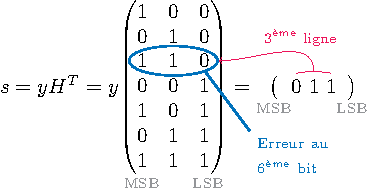
\includegraphics[scale=1]{drwg_6.pdf}
\end{center}
Cette façon de faire permet d'éliminer les éventuelles erreurs due à l'ordre de construction de la matrice (LSB en haut ou LSB en bas).\\
Ceci fonctionne \textbf{uniquement} avec la matrice de Hamming (dont les lignes sont 1,2,3... en binaire). Si on regarde la matrice non-transposée ce sera les colonnes



\subsection{Propriétés}
$$G_SH_S^T=0$$
\subsection{Codes polynomiaux}
\begin{enumerate}
\item Souvent linéaires (+ parfois cycliques)
\item Générateur rarement systématique (on peut utiliser un encodage systématique si le générateur ne l'est pas)
\end{enumerate}
\subsection{Codes linéaires}
La somme de deux codes valides donne un nouveau code valide
\subsection{Codes cycliques}
Un décalage vers la gauche $\textcolor{OrangeRed}{0}011\longrightarrow 011\textcolor{OrangeRed}{0}$ ou vers la droite $001\textcolor{OrangeRed}{1}\longrightarrow \textcolor{OrangeRed}{1}001$ donne un autre code valide.\\
Un décalage d'un mot-code de longueur $n$ dans $\mathbb{R}_n[X]$ est similaire à une multiplication par $X$.\\
Si $g(x)$ est un facteur de $1+X^n$ alors le code est cyclique.
\subsubsection{Générateur}
Un générateur permet, par des décalages cycliques et des sommes d'obtenir tous les mots-code.\\
Si le générateur divise $(1+X^n)$ alors le code est cyclique
\subsubsection{Encodage}
On veut encoder un message $x$ et obtenir le mot-code $y$
\paragraph{Encodage systématique} :
$$x\xrightarrow{\text{encodage}} xX^{n-k}+\text{reste}\left(\frac{xX^{n-k}}{g(x)}\right)=y$$
Les bits du message se retrouvent au début du mot-code
\paragraph{Encodage "standard"} :
$$x\xrightarrow{\text{encodage}} xg(x)=y$$
\subsubsection{Vérification}
On va simplement chercher à savoir si le message est correct ou non.\\
Vérification systématique (on vérifie simplement que le message soit égal au reste, comme pour l'encodage)
$$y[0:k] == \text{reste}\left(\frac{y[0:k]X^{n-k}}{g(x)}\right)$$
Vérification "standard"
$$s(x)=e(x)=\frac{y}{g(x)}\qquad s(x)=0\longrightarrow\text{ ok}$$
\subsubsection{Correction d'erreurs}
On va utiliser une matrice de contrôle (typiquement pour les codes BCH) qui va indiquer la position de(s) erreur(s)
\subsubsection{Décodage}
Dans le cas où le message est correct, on va effectuer le décodage.\\
Décodage systématique (on récupère simplement les bits dans le message tels-quels):
$$\hat{x}=y[0:k]$$
Décodage "standard" :
$$\hat{x}=\frac{y}{g(x)}$$
\subsection{Générateur $\longrightarrow $ matrice}
\subsubsection{Non-systématique}
On peut créer la matrice en effectuant des décalages cycliques du générateur $g(x)$
$$\underset{k\times n}{\begin{pmatrix}
g_{k-1} & g_{k-2} & \cdots & g_{1} & g_0 & 0 & 0\\
0 & g_{k-1} & g_{k-2} & \cdots & g_{1} & g_0 & 0\\
 & & & \vdots\\
0 & 0 & g_{k-1} & g_{k-2} & \cdots & g_1 & g_0\\
\end{pmatrix}}$$
Fonctionne aussi si on mets le générateur dans l'autre sens.\\
\textcolor{OrangeRed}{A vérifier si valable en général (pas juste cyclique) mais en principe oui}.\\
Avec le nombre de lignes correspondant à la longueur du message. Cette matrice n'est pas systématique. Il faut la manipuler si on veut obtenir la version systématique. On effectue des combinaisons linéaires sur les lignes pour l'obtenir
\subsubsection{Systématique}
On prend des mots-codes et on les mets dans les lignes de la matrice. On choisi ces mots-codes pour qu'ils écrivent la matrice identité au début de $G_S$
$$G_S=\begin{pmatrix}
\text{Mot-code qui commence par } 1000\\
\text{Mot-code qui commence par } 0100\\
\text{Mot-code qui commence par } 0010\\
\text{Mot-code qui commence par } 0001
\end{pmatrix}$$
\subsection{Codage convolutionnel}
Construire une table pour déterminer les états futurs (Avec 3 délais)
\begin{center}
\begin{tabular}{cccccc}
$t$ & $U$ & $D_0$ & $D_1$ & $D_2$ & $Y$\\\hline
0 & $u_{k-1}$ & 0 & 0 & 0 & 0\\
1 & $u_{k-2}$ & $u_{k-1}$ & $\cdots$ & & $0$\\
$\vdots$ & & & & &  $\vdots$\\
$k-2$ & $u_1$ & & & & $q_1$\\
$k-1$ & $u_0$ & & & & $q_0$\\\hline
$k$ & $0$ & $r_0$ & $r_1$ & $r_2$
\end{tabular}
\end{center}
Le reste se retrouve sur les mémoires lorsqu'on a terminé d'envoyer le message
\end{document}